% !TEX program = xelatex
\documentclass[11pt]{article}

\usepackage{fontspec}
\usepackage{unicode-math}
\setmainfont{Latin Modern Roman}
\setsansfont{Latin Modern Sans}
\setmonofont{Latin Modern Mono}[Scale=0.88]
\usepackage{xeCJK}
\setCJKmainfont{Droid Sans Fallback}
\setCJKsansfont{Droid Sans Fallback}
\setCJKmonofont{Droid Sans Fallback}

\usepackage{graphicx}
\graphicspath{{figures/}{../../papers/arxiv-ac/figures/}}
\usepackage{booktabs}
\usepackage{tabularx}
\usepackage{ragged2e}
\usepackage{microtype}
\usepackage{natbib}
\usepackage{listings}

\makeatletter
\def\input@path{{../}}
\makeatother
\usepackage{ac-paper-cards}

\hypersetup{
  pdftitle={可演奏的民歌：口头传统遇上浏览器键盘},
}

% Listing style for notepat song notation
\lstdefinestyle{notepat}{
  basicstyle=\ttfamily\small,
  breaklines=true,
  columns=flexible,
  keepspaces=true,
  showstringspaces=false,
}

\begin{document}

% ============================================================
% TITLE CARD
% ============================================================
\thispagestyle{empty}
\vspace*{\fill}
\begin{center}
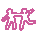
\includegraphics[height=3em]{pals}\par\vspace{0.6em}
{\acbold\fontsize{20pt}{24pt}\selectfont\color{acdark} 可演奏的}\par
{\acbold\fontsize{20pt}{24pt}\selectfont\color{acdark} 民歌}\par
\vspace{0.3em}
{\aclight\fontsize{10pt}{12pt}\selectfont\color{acpink} 口头传统遇上浏览器键盘}\par
\vspace{0.8em}
{\normalsize\href{https://prompt.ac/@jeffrey}{@jeffrey}}\par
{\small\color{acgray} Aesthetic.Computer}\par
{\small\color{acgray} ORCID: \href{https://orcid.org/0009-0007-4460-4913}{0009-0007-4460-4913}}\par
\vspace{0.3em}
{\small\color{acpurple} \url{https://notepat.com}}\par
\vspace{0.8em}
\rule{0.6\textwidth}{1pt}\par
\vspace{0.4em}
{\small\color{acpink}\textbf{[ 工作草稿 able---请勿引用 ]}}\par
\vspace{0.3em}
{\footnotesize\color{acgray} 2026年3月}\par
\end{center}
\vspace*{\fill}

% ============================================================
% ABSTRACT CARD
% ============================================================
\clearpage
\begin{accentcard}
\cardtitle{摘要}

民歌的演化使其无需记谱即可演奏，无需乐器即可记忆，无需许可即可改编。这些特性——有限的音域、重复的结构、口头可传播性——使民歌旋律在结构上非常适合基于浏览器的键盘合成器。

\vspace{0.3em}

本文描述了将可演奏民歌整合到 \np{}.com 中的过程。\np{} 是一款半音阶键盘乐器，将 QWERTY 键映射到音符。我们使用轻量级的 \texttt{NOTE:word} 格式编码民歌旋律，将每个音高与其歌词音节配对，从而创建一种引导演奏模式，让乐器逐个音符地教授歌曲。

\vspace{0.3em}

我们调查了适合此编码方式的民歌旋律集合，分析了民歌的结构约束为何与键盘即乐器的界面相匹配，并论证了民歌过程——变异、选择、口头传播——在可通过 URL 分享和复刻的歌曲编码中有着天然的数字对应物。
\end{accentcard}

% ============================================================
% SECTION 1: THE ARGUMENT
% ============================================================
\section{论点}

民歌是人类最古老的开源软件。

它们没有单一的作者。它们由社区维护。它们通过口头传播——这意味着它们必须足够简单以便记忆，足够受限以便复现，又足够灵活以便适应。每一位歌者都是贡献者；每一次演唱都是一次复刻。

\vspace{0.3em}

这些恰恰是使旋律可以在 QWERTY 键盘上演奏的特性。

\begin{card}
\cardtitle{为什么选择民歌？}
\begin{itemize}
  \item \textbf{狭窄的音域}：大多数民歌旋律跨越 1--1.5 个八度~\citep{lomax1968folk}。\np{} 的双八度按钮网格可以完全覆盖它们。
  \item \textbf{五声音阶倾向}：许多传统偏好五音音阶~\citep{kodaly1971folk}，减少了寻找下一个音符的认知负担。
  \item \textbf{重复的结构}：重复的8小节乐句、呼应模式、主歌-副歌形式——这些都有助于记忆和引导式回放。
  \item \textbf{没有错音}：在五声音阶旋律中，相邻的音阶音是协和的。Orff Schulwerk 方法利用了同样的特性，通过可拆卸的木琴音条来实现~\citep{orff1978schulwerk}。
\end{itemize}
\end{card}

% ============================================================
% SECTION 2: THE INSTRUMENT
% ============================================================
\section{乐器}

\np{}.com 是一款基于浏览器的半音阶合成器，作为 \ac{} 中的一个"piece"（交互式程序）构建~\citep{scudder2026ac, scudder2026notepat}。它将 QWERTY 键盘映射到跨越两个八度的24个半音音符，通过八度切换可覆盖完整的钢琴音域。

\begin{darkcard}
\textbf{歌曲模式}将 \np{} 从自由演奏乐器转变为引导式演奏界面。滚动的歌词轨道显示当前音节；只有正确的音符处于激活状态；按下它即可前进到下一个音节。演奏者不可能犯错——只能等待。
\end{darkcard}

这种"辅助轮"方式——阻止错误的音符、高亮正确的音符——呼应了 Orff 和 Kod\'aly 教学法，它们通过限制乐器来匹配学习者当前的能力~\citep{kodaly1971folk, orff1978schulwerk}。

% ============================================================
% SECTION 3: THE ENCODING
% ============================================================
\section{编码方式}

\np{} 中的歌曲被编码为以空格分隔的 \texttt{NOTE:word} 配对：

\notesong{C:Twin- C:-kle G:twin- G:-kle A:lit- A:-tle G:star,\\
F:how F:I E:won- E:-der D:what D:you C:are.}

每个标记是一个音符名称（\texttt{C}、\texttt{G}、\texttt{A}、\texttt{F\#} 等）通过冒号与歌词音节配对。连字符表示音节的延续：尾部连字符（\texttt{Twin-}）表示下一个标记继续同一个单词；头部连字符（\texttt{-kle}）是延续部分。

\begin{card}
\cardtitle{设计特性}
\begin{itemize}
  \item \textbf{人类可读}：音乐家可以直接视读该编码。
  \item \textbf{URL安全}：歌曲可以作为 URL 参数传递给 \np{}。
  \item \textbf{可复刻}：复制、编辑、分享——文本字符串中的民歌过程。
  \item \textbf{极简}：没有时值，没有力度，没有速度。这三者都由演奏者控制。
\end{itemize}
\end{card}

缺少节奏信息是刻意为之。在口头传统中，节奏属于表演者，而非乐谱~\citep{lomax1968folk}。编码捕捉的是\emph{演奏什么}；演奏者决定\emph{如何演奏}。

% ============================================================
% SECTION 4: A CATALOG
% ============================================================
\section{可演奏旋律目录}

我们调查了来自多种传统的民歌集合，选择了针对 \np{} 双八度网格优化的旋律。选择标准：音域 $\leq$\,15个半音、五声音阶或简单全音阶、以及文化辨识度。

\begin{card}
\cardtitle{五声音阶（5个音符）}
\begin{tabularx}{\linewidth}{Xll}
\toprule
\textbf{歌曲} & \textbf{起源} & \textbf{音域} \\
\midrule
Amazing Grace & 美国 & P5+oct \\
Auld Lang Syne & 苏格兰 & oct \\
Arirang & 韩国 & oct \\
Sakura & 日本 & m7 \\
Mo Li Hua（茉莉花） & 中国 & oct \\
Swing Low & 灵歌 & oct \\
\bottomrule
\end{tabularx}
\end{card}

\begin{card}
\cardtitle{窄音域（小于一个八度）}
\begin{tabularx}{\linewidth}{Xll}
\toprule
\textbf{歌曲} & \textbf{起源} & \textbf{音域} \\
\midrule
Mary Had a Little Lamb & 美国 & P5 \\
Hot Cross Buns & 英国 & M3 \\
Fr\`ere Jacques & 法国 & M6 \\
London Bridge & 英国 & P5 \\
Korobeiniki & 俄国 & oct \\
\bottomrule
\end{tabularx}
\end{card}

\begin{card}
\cardtitle{调式与全音阶}
\begin{tabularx}{\linewidth}{Xll}
\toprule
\textbf{歌曲} & \textbf{起源} & \textbf{音域} \\
\midrule
Greensleeves & 英国 & 10th \\
Scarborough Fair & 英国 & oct \\
Danny Boy & 爱尔兰 & 10th \\
Shenandoah & 美国 & 10th \\
Hava Nagila & 以色列 & oct \\
\bottomrule
\end{tabularx}
\end{card}

% ============================================================
% SECTION 5: FOLK PROCESS AS VERSION CONTROL
% ============================================================
\section{民歌过程即版本控制}

国际民间音乐委员会确定了民歌过程的三个特性：\emph{连续性}（将现在与过去联系起来）、\emph{变异}（个体表演者的创造性冲动）和\emph{选择}（社区决定哪些形式存续）~\citep{karpeles1955definition}。

\begin{accentcard}
这些直接对应于软件版本控制：

\vspace{0.3em}
\begin{tabularx}{\linewidth}{lX}
\textbf{连续性} & \texttt{main} 分支 \\
\textbf{变异} & 提交、复刻 \\
\textbf{选择} & 合并决策、采纳 \\
\end{tabularx}
\end{accentcard}

一首 \np{} 歌曲编码就是一个 URL。分享一首歌就是分享一个链接。修改一首歌就是编辑一个文本字符串并分享一个新链接。"口头传统"变成了 URL 的传统——旋律不再通过记忆传播，而是通过超文本传播。

这并非隐喻。Essen 关联码（ESAC）数据库始建于1982年，以受中国\textit{简谱}启发的计算机友好记谱法编码了约8,000首欧洲和中国民歌~\citep{schaffrath1995esac}。\np{} 的 \texttt{NOTE:word} 格式是这一传统的直接后裔：将旋律编码为文本，使计算和传播成为可能。

% ============================================================
% SECTION 6: COMPUTATIONAL MUSICOLOGY
% ============================================================
\section{计算维度}

Passmore 等人将民歌旋律建模为来自12音"字母表"的演化序列，将借鉴自分子遗传学的序列比对方法应用于10,062首日本和英国旋律~\citep{passmore2023cultural}。他们发现，旋律影响较小的音符变化更可能存续——这种选择压力有利于民歌所著称的简洁性。

\begin{card}
\cardtitle{这对 \np{} 意味着什么}

如果民歌旋律受到趋向简洁的演化选择压力，那么它们正在\emph{收敛}于使其可在受限界面上演奏的那些特性。QWERTY 键盘不是钢琴的贫乏替代品——它是一种约束，与民歌过程已经施加的约束相匹配。
\end{card}

Lomax 的歌唱测量学项目对来自1,026个社会的5,776首歌曲的37个表演风格方面进行了编码，发现表演风格（而非旋律内容）是主要的文化指标~\citep{lomax1968folk}。这支持了 \np{} 编码音高但不编码节奏的设计决策：文化上有意义的变异发生在音符\emph{如何}被演奏上，而这恰恰是演奏者所控制的。

% ============================================================
% SECTION 7: RELATED INSTRUMENTS
% ============================================================
\section{相关乐器}

\begin{card}
\cardtitle{aQWERTYon}
纽约大学音乐体验设计实验室构建了 aQWERTYon，一款将 QWERTY 键映射到音阶度数的浏览器乐器，从而实现"没有错音"~\citep{hein2017aqwertyon}。\np{} 在两个方面有所不同：它使用\emph{半音阶}映射（错音是可能的，且具有教学价值），并且将音符与歌词配对（歌曲自我教授）。
\end{card}

\begin{card}
\cardtitle{ABC Notation}
ABC notation 是民歌音乐编码的事实标准，以文本形式表示旋律~\citep{walshaw2011abc}。\texttt{abcjs} 库将 ABC 渲染为浏览器中的交互式乐谱。\np{} 的编码更简单——没有时值，没有小节线——因为它不是一个记谱系统，而是一个\emph{演奏脚本}：它告诉演奏者按什么键，而不是音乐看起来像什么。
\end{card}

\begin{card}
\cardtitle{Tunepal}
一个音乐信息检索系统，通过"以演奏查询"的方式将音乐家与13,290首传统爱尔兰曲调连接起来~\citep{duggan2009tunepal}。Tunepal 找到曲调；\np{} 教授它们。二者是互补的。
\end{card}

% ============================================================
% SECTION 8: THE BARE-METAL FOLK INSTRUMENT
% ============================================================
\section{裸金属民间乐器}

\np{} 不仅在浏览器中运行，还在裸金属上运行——一个987行的 QuickJS 移植版本，作为 PID~1 在 AC Native OS 上启动~\citep{scudder2026os}。一台在裸金属上运行 \np{} 的笔记本电脑，从字面意义上来说，就是一件民间乐器：一个用于演奏歌曲的单一用途设备，没有操作系统，没有桌面，没有干扰。

\begin{accentcard}
融合已经完成：民歌，被设计为在最简单的可用乐器上演奏，运行在最简单的可能计算机上——一个 Linux 内核、一个帧缓冲区和一个键盘。
\end{accentcard}

% ============================================================
% SECTION 9: FUTURE WORK
% ============================================================
\section{未来工作}

\begin{card}
\begin{itemize}
  \item \textbf{众包编码}：一个公开的 \texttt{NOTE:word} 编码仓库，以 URL 形式提交，像民歌本身一样进行版本管理。
  \item \textbf{跨文化集合}：将 Essen、Roud 和 Lomax 档案中的旋律编码为 \np{} 格式，获得许可并注明出处。
  \item \textbf{自适应难度}：随着演奏者掌握更简单的歌曲，逐步扩大音域——一种类似 Kod\'aly 的民歌曲目渐进方式。
  \item \textbf{多人民歌会}：两位 \np{} 演奏者演奏同一首歌，一人演奏旋律，一人演奏和声——爱尔兰传统意义上的数字"聚会"。
  \item \textbf{录音与分享}：将演奏捕捉为音频，与编码 URL 配对并发布——一种有据可查的口头传统。
\end{itemize}
\end{card}

% ============================================================
% CONCLUSION CARD
% ============================================================
\section{结论}

民歌在没有记谱、没有录音、没有乐器的情况下存续了数个世纪。它们之所以存续，是因为它们足够简单以便记忆，足够灵活以便适应，又足够有价值以便分享。

一个逐个音符教授这些歌曲的浏览器键盘，并非对民歌传统的偏离。它\emph{就是}民歌传统——再一次适应了手边的乐器。

\vspace{0.5em}
\noindent\textbf{ORCID:} \href{https://orcid.org/0009-0007-4460-4913}{0009-0007-4460-4913}

\bibliographystyle{plainnat}
\bibliography{references}

\end{document}
